\section{Discussion}
\label{sec:c5_discussion}

\subsection{Comparison to Observed \Mtot-\MNi\ Relations}
\label{ssec:c5_comparetoobs}

\begin{figure}
\centering
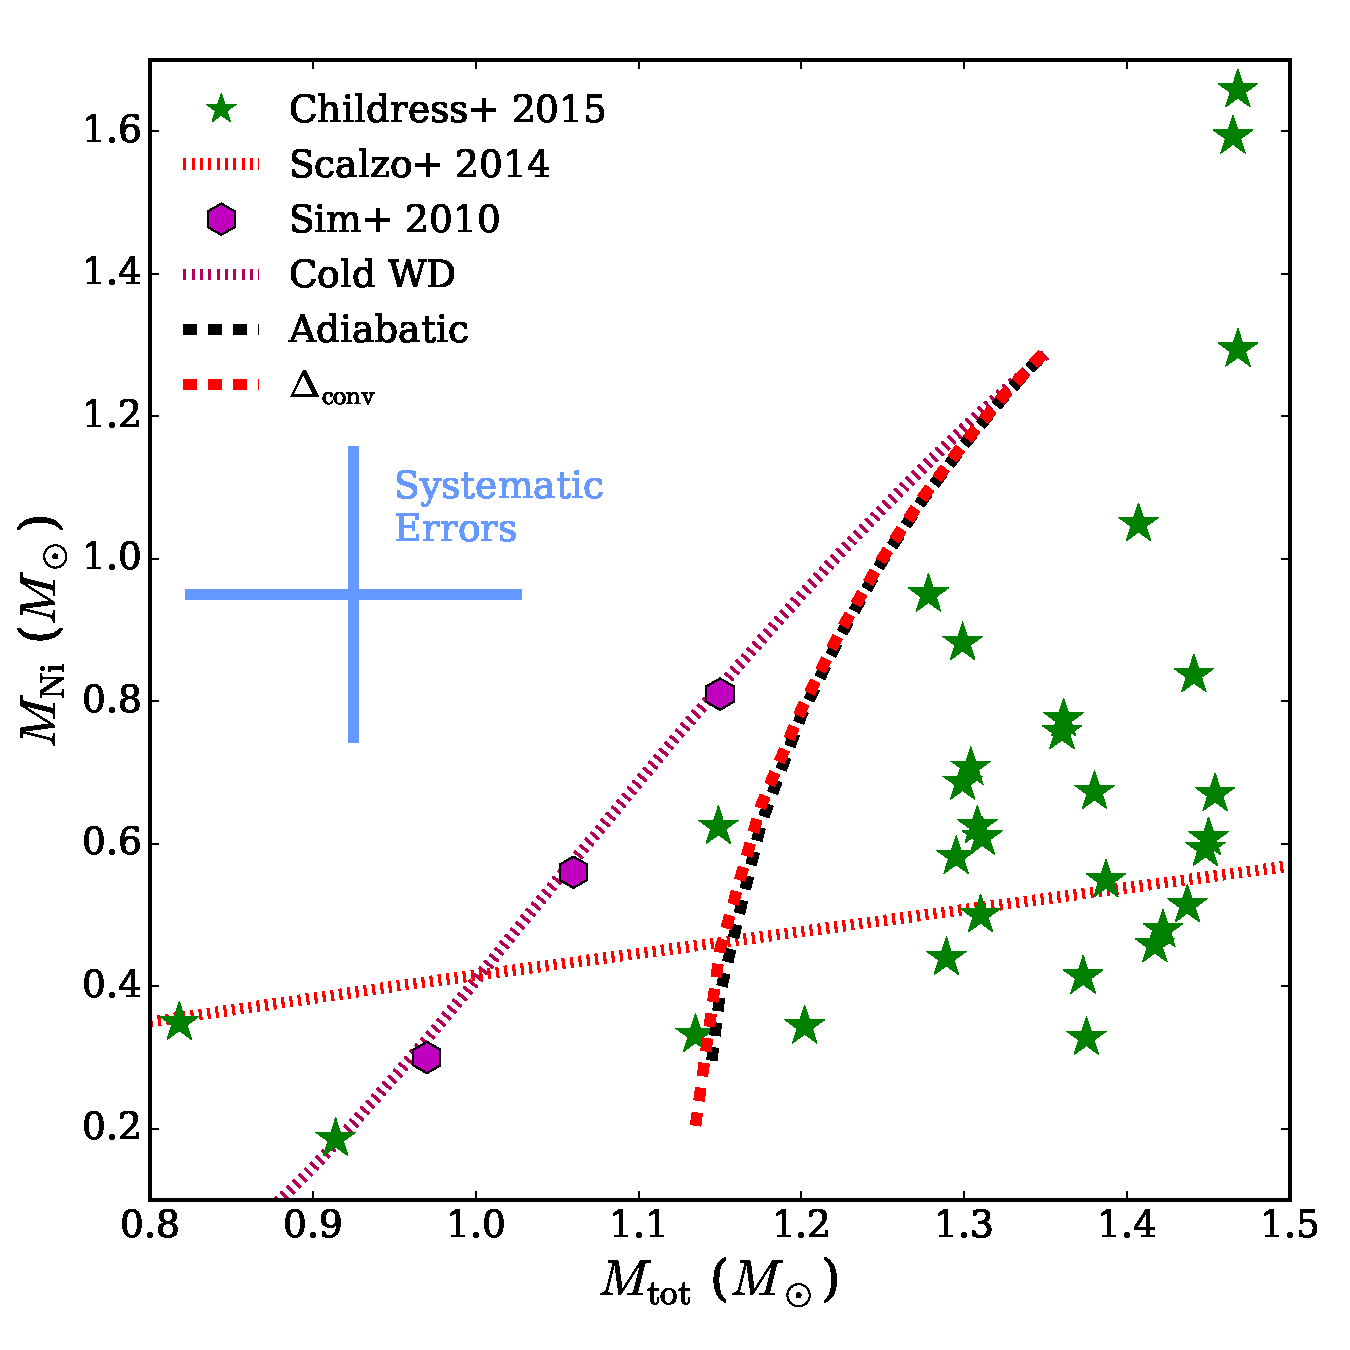
\includegraphics[angle=0,width=0.8\columnwidth]{chapter5_zhu+16/figures/mni.pdf}
\caption{Relationships between total ejected mass \Mtot\ and synthesized \Ni\ mass \MNi\ for adiabatic and \dnabconv-inclusive WDs that experience a pure detonation immediately after the end of simmering, estimated using \cite{sim+10}.  Also plotted are the \Mtot\ and \MNi\ yields of $31$ observed SNe Ia from \cite{chil+15}, and the relationship derived by \cite{scalzrs14} from 337 observed SNe Ia.  \cite{chil+15}'s systematic error bars, indicating how much their values can be shifted in unison, are also included.  The dashed magenta line is the relationship for the pure detonation of cold (uniform $10^5$ K) WDs, with the simulation results of \cite{sim+10} overdrawn.}
\label{fig:c5_mni}
\end{figure}

%Colors indicate adiabatic approximation, inclusion of \dnabconv, low ($\EBEtot = 2.9\times10^{-5}$) or high ($\EBEtot = 2.8\times10^{-3}$ magnetic field, or solid-body rotation.

We have estimated the range of masses of centrally-simmering sub-\Mch\ WDs that explode, as well as their corresponding \MNi\ yields assuming a pure detonation immediately after simmering.  Putting aside the possibility that extremely strong magnetic fields could affect \vconv, we have also determined that this range does not significantly change when including \dnabconv, rotation or magnetic fields.  It is then interesting to consider in the abstract whether these could reproduce a substantial portion of the SN Ia parameter space, and, to that end, we compare our results to estimates of ejected mass and \Ni\ yields for observed SNe Ia.  In Fig. \ref{fig:c5_mni}, we plot the $\MNi-\Mtot$ relationship for adiabatic and \dnabconv-inclusive WDs, as well as the relationship (also derived using $M(\rho>10^7)$) from the pure detonation of uniform $10^5$ K cold WD for comparison.  Additionally, results from the pure detonation simulations of \cite{sim+10} are plotted to show the accuracy of the $M(\rho>10^7)$ estimate.  Alongside these, we plot the best-fit relationship to the ejected and synthesized \Ni\ masses of $337$ observed ``normal'' \citep{bran+06} SNe Ia from \cite{scalzrs14}, and the estimated \Mtot\ and \MNi\ of $31$ normal SNe Ia from \cite{chil+15}.  \cite{scalzrs14} derives their $\MNi-\Mtot$ relationship from the observed bolometric light curve (using a range of simulated explosion models as priors; \citealt{scalz+14}), and \cite{chil+15} use \cite{scalzrs14}'s method of estimating \Mtot\ while obtaining \MNi\ from the evolution of the $[\textsc{Co\,III}]$ $\lambda5893$ emission complex during the SN Ia nebular phase.

%peak luminosity and decline rate
%, WDs with weaker ($\EBEtot = 2.9\times10^{-5}$) or stronger ($\EBEtot = 2.8\times10^{-3}$ magnetic fields and 50\% critically rotating

As expected from previous analysis, the $\MNi-\Mtot$ relationship changes little between the adiabatic and \dnabconv-inclusive WDs, being separated by a $\Mtot\lesssim0.01\,\Msun$ for any given \MNi.  While not plotted, we also found that this is true for WDs rotating at $50$\% of critical, and those with $\sim10^{11}\,\mrm{G}$ magnetic fields.  The previously-noted steep dependence of \MNi\ on \Mtot\ near \Mcrit\ is clear as well: a linear fit around $\Mtot = 1.15\,\Msun$ gives $d\MNi/d\Mtot \approx 10$ (for both curves), making it difficult to accurately estimate a minimum \MNi.  This also leads to a fine-tuning problem: to produce \MNi\ between $\sim0.3-0.6\,\Msun$ -- typical \MNi\ yields in \cite{scalzrs14} and \cite{chil+15} -- requires \Mtot\ to lie in a narrow range between $\sim 1.13 - 1.17\,\Msun$.  It is not obvious why a progenitor channel would favor this mass range, though we note the distribution of field CO WD masses is very narrowly peaked (at $0.65\,\Msun$; eg. \citealt{tremb09, klei+13}), possibly indicating that merging CO WD binaries masses fall within a narrow range.

%The simple estimate in \citeal{zhu+13}, for example, the combined mass of material in the degeneracy supported core and and thermally supported hot atmosphere -- the ``core-envelope mass'' -- is broadly distributed from $\sim 0.7 - 1.2\,\Msun$ ($\sim70 - 80$\% the mass of the accreting WD) across the mass parameter space of merging CO WDs.  

%ven if we relax the relationship to the space bounded by the Cold WD and simmering WD lines.

Nevertheless, the $\MNi-\Mtot$ relationship from pure detonations of centrally simmering CO WDs does not resemble the observed ones.  \cite{chil+15}'s values could be systematically offset by $\sim 0.1\,\Msun$ in \Mtot\ and $\sim 0.2\,\Msun$ in \MNi, but these apply to the points as a whole, and we also do not reproduce the shape of \cite{chil+15}'s distribution.  This issue is not unique to our work - \cite{scalzrs14} and \cite{chil+15} plot theoretical $\MNi-\Mtot$ curves for a wide range of proposed SN Ia progenitor classes, ranging from sub-\Mch\ WDs undergoing a double-detonation (equivalent to the Cold WD line in Fig. \ref{fig:c5_mni}) to \Mch\ pure deflagrations, and find no individual class able to reproduce the entire observed $\MNi-\Mtot$ parameter space.  If their results indeed reflect the true \Mtot-\Ni\ relationship of SNe Ia, either multiple progenitor channels are necessary, or a novel understanding of progenitors must arise.

% , an existing channel is improperly understood, or a new channel that is able to span the space must be proposed.

\subsection{Implications for Mergers as SN Ia Progenitors}
\label{ssec:c5_implications}

Regardless of whether simmering sub-\Mch\ WDs can reproduce observations, what implications do our results have on double-degenerate CO WD mergers as SN Ia progenitors, in particular the channel of \citeal{vkercj10} involving sub-\Mch\ merger remnants that ignite central nuclear fusion following their viscous evolution?  A direct mapping of post-viscous remnants onto our hydrostatic simmering WDs is not possible since their structures are quite complex, and in general their temperature profiles are substantially shallower than the convective ones used in our models.  Moreover, much of their mass exists as a hot, tenuous envelope that surrounds and exerts little pressure support on their dense, degeneracy-supported ``cores''.  As a rough estimate, we can consider the evolution of these cores as separate from their envelopes (the transition region between the two might resemble the hot atmospheres in Sec. \ref{sssec:c5_runaway_ad_hot}, and thus not affect the core's evolution).

Regardless of their initial conditions, the simmering tracks of a remnant core cannot simultaneously increase in temperature and density, since this would require part of their structure to cool (Sec. \ref{ssec:c5_numericalmodels}).  They also cannot exist, for longer than a few convective timescales, to the right of the rising portion of the simmering track of the same mass in Fig. \ref{fig:c5_runaway_rhot}, i.e. the portion of the track between the start of simmering and either the end of simmering point or the point of maximum temperature.  Doing so would mean its temperature gradient has become steeper than the convective one, and convective energy transport will rapidly lower the gradient back to the convective one (like for stars to the right of the Hayashi track).  As a consequence of these two restrictions, \Mcrit\ will increase for those WDs with shallow temperature profiles.  With this in mind, meaningful conclusions can be made by examining the central densities and core masses \Mc\ of post-viscous remnants.

%A direct mapping of the remnants of CO WD mergers onto hydrostatic WDs with (super)-adiabatic profiles is difficult, since these remnants will first undergo viscous redistribution of angular momentum over $10^4-10^8\,\mrm{s}$, and potentially a period of thermal evolution over $\sim10^4\,\mrm{yr}$, before igniting fusion \citep{shen+12}.  Post-viscous CO-CO remnant density and temperature profiles have been calculated for a $0.6 - 0.9\,\Msun$ remnant \citep{schw+12} and for a $0.6 - 0.6\,\Msun$ one \citep{ji+13}.  The former ignites non-degenerate carbon fusion far from the remnant center, which cannot be represented by our models, and will likely produce an oxygen-neon WD \citep{shen+12}.  The latter does ignite partly degenerate carbon fusion, but has a temperature profile that is substantially shallower than adiabatic, and so cannot simply be transliterated to a cold WD with a hot atmosphere.

To our knowledge, the sole published viscous evolution simulation of a sub-\Mch\ double CO WD merger remnant is that of \cite{ji+13}.  They find, by the end of their simulation, the central density and temperature of their $0.6 - 0.6\,\Msun$ remnant are $\sim5\times10^6\,\gcc$ and $\sim9\times10^8\,\mrm{K}$, respectively, well above the $\taucc = \taunu$ line.  Indeed, its $\taucc \sim 1\,\mrm{yr}$, much smaller than the $\gtrsim 10^4\,\mrm{yr}$ thermal contraction timescale \citep{shen+12}, so the remnant will begin to simmer.  The mass of the remnant that is within $r = 1.5\times10^9\,\mrm{cm}$ (the approximate outer boundary of the dense core in \citealt{ji+13} Fig. 1) is $\sim1.07\,\Msun$ (Suoqing Ji and Robert Fisher private communication, 2016), $\sim0.06\,\Msun$ lower than \Mcrit.  The remnant's central density is a factor of $\sim4$ lower than that for the $\sim1.05\,\Msun$ simmering track at the same temperature and a factor of $\sim6$ lower than that for the \Mcrit\ simmering track.\footnote{The remnant in \citep{ji+13} has not lost all of its rotational support by the end of their simulation, so its central density will continue to increase early in its simmering phase.  As less than a third of its initial angular momentum remains, however, it is unlikely to increase by a factor of $\sim4$.}  The most likely fate of this system is therefore expansion and possibly stable nuclear burning.  The relatively small difference between \Mc\ and \Mcrit\ suggests a merger remnant $\sim0.1\,\Msun$ more massive might possess a core mass in excess of \Mcrit.  That core's central density, though, may still be too low for simmering to end in an explosion.

%an order of magnitude lower than the \rhoc\ of any simmering tracks considered in Sec. \ref{sec:results}.

% It is thus almost certainly going to become non-degenerate and expand at temperatures well below those for dynamical burning.

For a broader parameter space of post-viscous remnants, we turn to the simple estimate of viscous evolution outcomes made in Sec. \ref{sec:c2_postmerger}.  While it tends to overestimate compression, particularly for remnants from similar-mass mergers, when compared to \citeauthor{schw+12} (and follow-up work in \citealt{rask+14}) and \cite{ji+13}, it nevertheless gives a rough estimate of the post-viscous remnant parameter space.  Taking our estimate at face value, we find that only those remnants from mergers with primary WD masses above $\sim0.8\,\Msun$ have $\rhoc \gtrsim 3\times10^7\,\gcc$, which also suggests that only remnants with total masses above \Mch\ are likely to achieve dynamical burning following viscous spin-down.  Note that the most massive of these may have instead already exploded from extreme temperatures during their mergers (for primary WD masses $\gtrsim0.9\,\Msun$; \citealt{pakm+10,pakm+11}), or due to hydrodynamic instabilities immediately afterward (for primaries $\gtrsim1\,\Msun$; \citealt{kash+15}).

If explosion is in fact not possible following viscous evolution, then sub-\Mch\ remnants that ignite carbon fusion will experience expansion instead, and eventually possible stable nuclear burning as a carbon star.  Given their properties, they are candidate progenitors for isolated high-field magnetic WDs (eg. \citealt{garc+12}), in particular hot DQ WDs (\citealt{dunlc15,dunl15thesis} and references therein), which have hot, carbon-dominated atmospheres and appear to be massive, rapidly rotating and strongly magnetized.

%Examining similar-mass remnants -- as only these have hot cores -- in \citeal{zhu+13} Fig. 16, we find ignition is achieved only for those with primary WD masses above $\sim0.8\,\Msun$; these also have central densities $\rhoc \gtrsim 5\times10^7\,\gcc$, comparable to those found along the \Mcrit\ simmering track.  

% That last estimate comes from dr/dt = sqrt(2GM/r) -> r = (2GM)^(1/3)(3t/2)^(2/3)

%wherein we generated density and temperature profiles for post-viscous remnant cores by assuming that all the remnant's angular momentum is carried away to large distance, the corresponding material forms a tenuous hot atmosphere with zero total energy, and material not carried away retains its original entropy

%Prad/Pion \propto T^3/\rho \propto \rho in adiabatic envelopes; we're in general much colder for any given density than Shen+12, so our radiation-dominated sparse atmosphere comes from magnetic reconnection (ji+13), while Shen's comes from an adiabatic non-degenerate envelope.

%This result poses a problem for the \citeal{vkercj10} sub-\Mch\ merger channel.  \cite{shen+12} finds further compression could occur during the subsequent \textit{thermal} evolution of the remnant over $\gtrsim10^4\,\mrm{yr}$, which may allow more remnants to reach higher central density and enclose more mass within their cores.  Whether central burning could still begin is uncertain, however, since thermal diffusion and neutrino-driven cooling may favor off-center carbon ignition, or simply net cooling, even for those post-viscous remnants that are initially $\gtrsim5\times10^8\,\mrm{K}$ at their center.  Moreover, remnants, with radiation-dominated and highly magnetized carbon atmospheres, will likely drive strong outflows during their thermal evolution, further complicating predictions.  We note one advantage for delaying the explosion to during thermal evolution is the removal of the ``clutter'' of the $\gtrsim0.1\,\Msun$ hot envelope surrounding the core and extending out to $\gtrsim10^{11}\,\mrm{cm}$ \citep{shen+12}.  This imparts signatures onto the explosion not seen in ordinary SNe Ia, such as a double-peaked light curve from the shock cooling of the envelope, excess blue and UV emission prior to peak light, and a slow-decaying light curve near peak light \citep{frye+10,levasg15,pirom15}.  While \cite{shen+12}'s simulation suggests thermal evolution will do little to alter the overall structure of the envelope \citep{pirom15}, it does not account for mass loss due to winds.  These will significantly alter the size and structure of the envelope, perhaps mitigating its effects on any eventual explosion.  Meanwhile, material ejected from the remnant (both during its viscous and subsequent thermal phases) moving at the escape velocity will approach $\sim10^{17}\,\mrm{cm}$ after $\sim10^4\,\mrm{yr}$.  Interaction between this material and light from the supernova could explain \citep{shen+12, ji+13} observations of SN Ia-CSM interactions such as time-variable NaID lines (eg. \citealt{pata+07, simo+09}).

\subsection{Accuracy of Magnetized Simmering Models}
\label{ssec:c5_magaccuracy}

We found in Sec. \ref{ssec:c5_rotmag} that $\lesssim10^{11}\,\mrm{G}$ magnetic fields negligibly affect simmering, while $\gtrsim10^{12}\,\mrm{G}$ ones could dramatically affect \vconv, but there are reasons to be cautious about these results, particularly in the strong field limit.

%and flow switches from steady convection to oscillatory motions along field lines.  The time averaged heat flux from these motions is much smaller

First, \citeal{stev79} does not include convective dynamo processes that amplify the magnetic field.  The vigorous convection zone found toward the end of simmering is an ideal environment for such processes -- analogous to the highly magnetized central convection zones of A and B main sequence stars (eg. \citealt{brunbt05, feat+09, augubt16}).  Amplification saturates when $\EBEconv \sim 1$, i.e. when, 

\eqbegin
B_\mrm{eq} \sim \vconv\sqrt{8\pi\rho}.
\eqend

\noindent For WDs at the end of simmering, $B_\mrm{eq} \sim 3\times10^{11}-1\times10^{12}\,\mrm{G}$.  These values match or exceed any magnetic fields generated by the merger or viscous evolution (though having fields in place at the start of simmering may increase the saturation field strength by up to another order of magnitude; \citealt{feat+09}), rendering even the low-field calculations uncertain.  Additionally, the turbulent nature of the dynamo will generate a highly tangled magnetic field that varies significantly over short length scales, unlike the large-scale fields assumed in this work; Eqn. \ref{eq:c5_dnabmag_est_work} would then suggest a much larger \dnabmag\ \citep{chabgb07}.

Second, studies of nonlinear magnetoconvection (eg. \citealt{procw82}) indicate that in steady state, magnetic fields are concentrated into high-flux bundles where the convective flow is truncated, surrounded by regions where convection continues uninhibited.  The amount of convective suppression depends on the volume fraction the bundles occupy.  When the ratio \EBEconv\ between magnetic and convective kinetic energy densities becomes higher than unity, the bundles merge and convection is effectively suppressed.  This physical picture (which is fundamentally multi-dimensional) shares little resemblance with \citeal{stev79} (Henk Spruit private communication, 2016), and no magnetic equivalent of \cite{barkdl14}'s examination of rotating convection has been conducted to see if \citeal{stev79} at least phenomenologically captures it.

%Note that $\EBEconv \ll 1$ for WDs with fields $\lesssim10^{11}\,\mrm{G}$, so this picture agrees with \citeal{stev79} that the convective flow is largely unimpeded, but this is only relevant if convective dynamo processes were inefficient.

%That said, $\EBEconv \ll 1$ for WDs with fields $\lesssim10^{11}\,\mrm{G}$ near the end of simmering, so this picture agrees with \citeal{stev79} that the convective flow is largely unimpeded.

Our model's inability to accurately follow magnetoconvection and include dynamo processes therefore constitutes the greatest uncertainty of this work.  While we have estimated that including rotation without magnetic fields is important only because it modifies the hydrostatic balance of the WD, rotation coupled with both convection and magnetic fields may additionally lead to unexpected emergent behavior.  The multidimensional nature of magnetoconvection may also alter the end of simmering criterion -- for example, if burning material is trapped within a flux bundle, it may locally run away and lead to dynamical burning even if convection is unhindered elsewhere in the WD.  We thus stress the need for more detailed investigation into WD magnetoconvection, potentially utilizing MHD convective simulations, in the future.

%In summary, we show that simple estimates of magnetoconvection when the field is $\lesssim10^{11}\,\mrm{G}$ will have a negligible effect on the runaway.  It is likely, however, that this field will grow considerably over the course of simmering due to convective (and likely rotational as well) dynamo processes, potentially reaching $\sim10^{12}\,\mrm{G}$, where our estimates both show more drastic changes to the convective velocity, and very likely break down.  Magnetoconvection in simmering WDs will have to be investigated with more detailed and likely simulation-based analysis.

%We can say, however, that if convective dynamo processes are inefficient in simmering WDs, then then our estimates become more believable in the case of a WD with a $\lesssim 10^{11}\,\mrm{G}$ magnetic field, , as $A \lesssim 1$ by the end of its simmering.

%A naive reading of the parameter space search e a parameter-space search for \Mcrit\ in this high-field limit yields a value $\sim0.1\,\Msun$ lower than at the low-field limit, the \citeal{wooswk04} is reached when the burning timescale is far longer than dynamical.
  

%and $\MNi = 0.21\,\Msun$

%However, we have already mentioned in Sec. \ref{ssec:magaccuracy} that these results, particularly those at the high-field limit, must be treated with caution.  \citeal{stev79}'s magnetic formulation has not yet been numerically tested and may not accurately reflect non-linear magnetoconvection, except perhaps in the case of weak fields.  Moreover, dynamo processes are likely to be efficient in simmering WDs and will likely lead to $\sim10^{12}\,\mrm{G}$ fields near the end of simmering, dominating over any fossil fields from prior evolution.


%In conclusion, we cannot constrain the magnetic field strength
%
% for two reasons.  First, studies of nonlinear magnetoconvection (eg. \citealt{procw82}) indicate that in steady state, fields are concentrated into bundles where the flow is truncated, surrounded by regions where convection continues uninhibited; convective suppression depends on the volume fraction the flux bundles occupy.  If magnetic dominates over convective energy density, the flux bundles merge and convection is effectively suppressed.  This picture bears little obvious resemblance to \citeal{stev79}'s formulation (Henk Spruit personal communication), and no equivalent to \cite{barkdl14} has been conducted to see if \citeal{stev79} is at least phenomenologically accurate.  The second and more important issue is that convective dynamo processes, neglected in our analysis, are likely to amplify any pre-existing magnetic fields by orders of magnitude during simmering.  The saturation field strength can be estimated by equating the magnetic and convective kinetic energy densities to obtain $B_\mrm{eq} \sim \vconv\sqrt{8\pi\rho}$.  For the WDs at the end of simmering, $B_\mrm{eq} \sim 3\times10^{11}-1\times10^{12}\,\mrm{G}$ (having strong fields in place at the start of simmering may increase these values by up to another order of magnitude; \citealt{feat+09}).  Coupling between convection and magnetic fields -- as well as rotation, in the most general case -- cannot be analyzed with \citeal{stev79}'s framework.  We therefore must leave investigation magnetoconvection to more detailed and likely simulation-based analysis methods.

%All this suggests that the fiducial 0.6-0.6\Msun merger proposed as a SN Ia progenitor by \cite{vkercj10} (and simulated by \cite{ji+13}) will expand and cool long before it achieves dynamical burning.  The remnants that can follow this simmering channel are likely to be similar-mass merger remnants whose total mass exceeds 1.8 Msun, which are rarer than even \Mch mergers (by definition!).

%The post-viscous evolution merger remnants of shen and ji, or the estimates from zhu+13, cannot directly be represented by spherically symmetric hydrostatic WDs.  Nevertheless, approximate translations can be made by either mapping the central density or mass which is degenerately supported into a simmering track.  the results of post-merger evolution studies like Application to Ji+13 results.  Further compression Badenes + Moaz for rare superchandra.

%-Should note in results section that having a hot atmosphere basically doesn't alter the interior.  Modifications to the temperature structure close to the centre of the remnant SHOULD do so, but only serve to lead to becoming nondegenerate earlier.

%It should first be noted that spun-down merger remnants cannot directly be mapped onto hydrostatic WDs with (super)-adiabatic profiles, since they tend to have more complex temperature profiles that are generally substantially shallower than adiabatic, and so cannot simply be represented by a cold WD with a hot atmosphere.  However, we can make rough comparisons, especially considering that in Sec. XXX, we noted that having a tenuous thermally supported atmosphere does little to alter the evolution of the simmering, degenerate core.  Post merger evolution simulations show that the final configuration of the spun-down remnant is indeed a degenerate core (cold or hot) surrounded by a tenuous atmosphere, and so we can map that cold degenerate core mass to a simmering track.  In Zhu+13, we make a rough estimate of the spun-down remnant profile, assuming that the rotational energy is dissipated entirely in the outer regions of the remnant, forming a hot atmosphere.  We find that about 75\% of the total mass of the remnant remains as a degenerate central object rather than a tenuous envelope, regardless of the mass ratio of the merging WDs.  This is supported by the simulations of Shen+12 of the PME of dissimilar mass merger remnants over a large range of total mass - they find the total mass within a cold core and a hot, isothermal plateau, to be 75\% the total mass (these all have cold cores, though, so wouldn't be represented by a center-lit runaway).  It is difficult to tell exactly what's going on in Ji's results, though an integration of the density profile within $10^9$ cm suggests a core mass of 0.8 Msun, somewhat lower than the 75\% we suggested.  If this 75\% thing holds, then only remnants of similar-mass mergers with total mass \textit{above} \Mch\ could form simmering cores above the critical mass.

%The estimate in zhu+13, and ji+13's results, also suggest the central density of the merger remnants of 0.65-0.65\Msun mergers is around 10**6.5, much lower than the \rhoc\ of the simmering \Mcrit\ WD at the same temperature.  Since \rhoc can only go down with increasing entropy, and being at lower \rhoc means being much closer to the degeneracy line, this system's evolution is highly likely to be expansion.

%We also do not consider the interplay between rotation, convection and magnetic field evolution, especially the growth of magnetic fields due to convective dynamos, and how they can be affected by the pre-existing field from the remnant.  As we found tentative evidence with our \citeal{stev79} estimate that field strengths on the order of $10^{12}\,\mrm{G}$, albeit larger than reasonable estimates for field strengths produced before or during simmering, may dramatically affect the convective velocity, this is a particularly interesting avenue of investigation.  The inherent complexity and multidimensional nature of the problem suggests that any future estimates of the temperature structure and convective velocity should be motivated by magnetohydrodynamic simulations of WD convection {\charles REFERENCES?}.  Finally, we use the analytic 1D dynamical burning criterion to determine the end of simmering, and a better estimate can be found by taking into account the range of temperatures and velocities individual convecting blobs may have (\citeal{wooswk04}) and how these can change because of, eg. magnetic fields altering the global convective flow patterns.
